\documentclass[]{article}
\usepackage{lmodern}
\usepackage{amssymb,amsmath}
\usepackage{ifxetex,ifluatex}
\usepackage{fixltx2e} % provides \textsubscript
\ifnum 0\ifxetex 1\fi\ifluatex 1\fi=0 % if pdftex
  \usepackage[T1]{fontenc}
  \usepackage[utf8]{inputenc}
\else % if luatex or xelatex
  \ifxetex
    \usepackage{mathspec}
    \usepackage{xltxtra,xunicode}
  \else
    \usepackage{fontspec}
  \fi
  \defaultfontfeatures{Mapping=tex-text,Scale=MatchLowercase}
  \newcommand{\euro}{€}
\fi
% use upquote if available, for straight quotes in verbatim environments
\IfFileExists{upquote.sty}{\usepackage{upquote}}{}
% use microtype if available
\IfFileExists{microtype.sty}{%
\usepackage{microtype}
\UseMicrotypeSet[protrusion]{basicmath} % disable protrusion for tt fonts
}{}
\usepackage[margin=1in]{geometry}
\usepackage{color}
\usepackage{fancyvrb}
\newcommand{\VerbBar}{|}
\newcommand{\VERB}{\Verb[commandchars=\\\{\}]}
\DefineVerbatimEnvironment{Highlighting}{Verbatim}{commandchars=\\\{\}}
% Add ',fontsize=\small' for more characters per line
\usepackage{framed}
\definecolor{shadecolor}{RGB}{248,248,248}
\newenvironment{Shaded}{\begin{snugshade}}{\end{snugshade}}
\newcommand{\KeywordTok}[1]{\textcolor[rgb]{0.13,0.29,0.53}{\textbf{{#1}}}}
\newcommand{\DataTypeTok}[1]{\textcolor[rgb]{0.13,0.29,0.53}{{#1}}}
\newcommand{\DecValTok}[1]{\textcolor[rgb]{0.00,0.00,0.81}{{#1}}}
\newcommand{\BaseNTok}[1]{\textcolor[rgb]{0.00,0.00,0.81}{{#1}}}
\newcommand{\FloatTok}[1]{\textcolor[rgb]{0.00,0.00,0.81}{{#1}}}
\newcommand{\CharTok}[1]{\textcolor[rgb]{0.31,0.60,0.02}{{#1}}}
\newcommand{\StringTok}[1]{\textcolor[rgb]{0.31,0.60,0.02}{{#1}}}
\newcommand{\CommentTok}[1]{\textcolor[rgb]{0.56,0.35,0.01}{\textit{{#1}}}}
\newcommand{\OtherTok}[1]{\textcolor[rgb]{0.56,0.35,0.01}{{#1}}}
\newcommand{\AlertTok}[1]{\textcolor[rgb]{0.94,0.16,0.16}{{#1}}}
\newcommand{\FunctionTok}[1]{\textcolor[rgb]{0.00,0.00,0.00}{{#1}}}
\newcommand{\RegionMarkerTok}[1]{{#1}}
\newcommand{\ErrorTok}[1]{\textbf{{#1}}}
\newcommand{\NormalTok}[1]{{#1}}
\usepackage{longtable,booktabs}
\usepackage{graphicx}
\makeatletter
\def\maxwidth{\ifdim\Gin@nat@width>\linewidth\linewidth\else\Gin@nat@width\fi}
\def\maxheight{\ifdim\Gin@nat@height>\textheight\textheight\else\Gin@nat@height\fi}
\makeatother
% Scale images if necessary, so that they will not overflow the page
% margins by default, and it is still possible to overwrite the defaults
% using explicit options in \includegraphics[width, height, ...]{}
\setkeys{Gin}{width=\maxwidth,height=\maxheight,keepaspectratio}
\ifxetex
  \usepackage[setpagesize=false, % page size defined by xetex
              unicode=false, % unicode breaks when used with xetex
              xetex]{hyperref}
\else
  \usepackage[unicode=true]{hyperref}
\fi
\hypersetup{breaklinks=true,
            bookmarks=true,
            pdfauthor={},
            pdftitle={HMM para reconocimiento de vocales},
            colorlinks=true,
            citecolor=blue,
            urlcolor=blue,
            linkcolor=magenta,
            pdfborder={0 0 0}}
\urlstyle{same}  % don't use monospace font for urls
\setlength{\parindent}{0pt}
\setlength{\parskip}{6pt plus 2pt minus 1pt}
\setlength{\emergencystretch}{3em}  % prevent overfull lines
\setcounter{secnumdepth}{5}

%%% Use protect on footnotes to avoid problems with footnotes in titles
\let\rmarkdownfootnote\footnote%
\def\footnote{\protect\rmarkdownfootnote}

%%% Change title format to be more compact
\usepackage{titling}
\setlength{\droptitle}{-2em}
  \title{HMM para reconocimiento de vocales}
  \pretitle{\vspace{\droptitle}\centering\huge}
  \posttitle{\par}
  \author{}
  \preauthor{}\postauthor{}
  \predate{\centering\large\emph}
  \postdate{\par}
  \date{18/05/2015}




\begin{document}

\maketitle


{
\hypersetup{linkcolor=black}
\setcounter{tocdepth}{2}
\tableofcontents
}
\pagebreak

\subsection{Introducción}\label{introduccion}

Los modelos de HMM son modelos estadísticos que se utilizan en procesos
que se suponen Markovianos donde los estados no son visibles
directamente ---son latentes--- pero las variables influidas por estos
estados si lo son. El objetivo consiste en identificar estos estados
ocultos para conocer los estados, las transiciones entre los estados y
las probabilidades de cada estado sobre las variables a las que
influyen.

Los HMM han sido ampliamente utilizados en problemas de Procesamiento de
Lenguaje Natural (NLP) sobre todo para el reconocimiento del habla (Part
Of Speech, POS), etiquetado gramatical, reconocimiento de escritura
manual, etc. Stamp (2012)

\subsection{Objetivo}\label{objetivo}

Identificación de vocales y consonantes de un texto en español a través
de un modelo de HMM estimando sus parámetros.

\subsection{Especificación del modelo}\label{especificacion-del-modelo}

\begin{itemize}
\itemsep1pt\parskip0pt\parsep0pt
\item
  Utilizamos HMM con el algoritmo Baum-Welch para estimar los
  parámetros:
\end{itemize}

\begin{enumerate}
\def\labelenumi{\arabic{enumi}.}
\itemsep1pt\parskip0pt\parsep0pt
\item
  las probabilidades inciales de los estados
\item
  las probabilidades de transición entre estados
\item
  las probabilidades de cada símbolo de pertenecer a uno de los estados
\end{enumerate}

\begin{figure}[htbp]
\centering
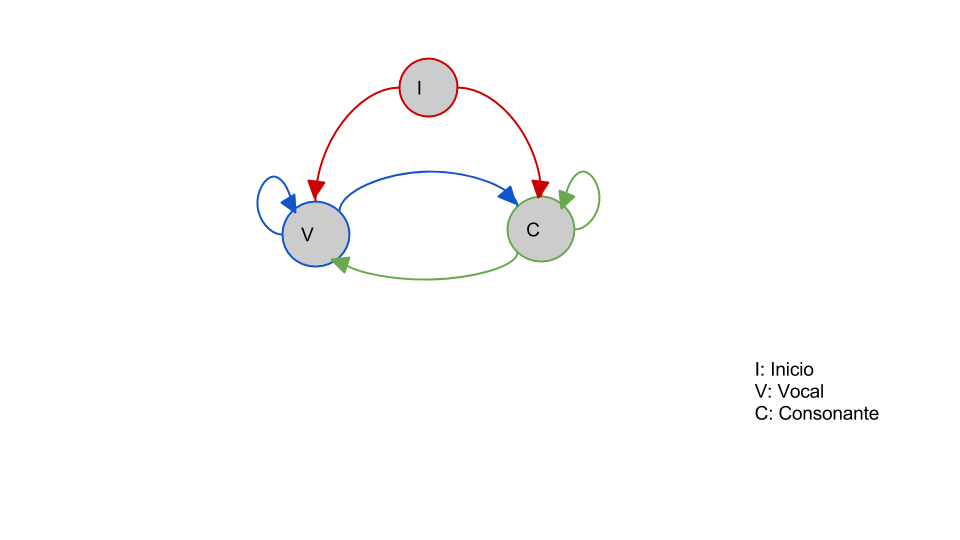
\includegraphics{modelo_vocales.png}
\caption{imagen}
\end{figure}

\subsubsection{Algoritmo Baum-Welch}\label{algoritmo-baum-welch}

\begin{itemize}
\itemsep1pt\parskip0pt\parsep0pt
\item
  Este algoritmo es una variante del EM visto en clase Frazzoli (2010);
  Bilmes (1998) . Iniciamos con un modelo sin `conocimiento'
\end{itemize}

$\pi$ = probabilidades de iniciar en cada estado

T= matriz de transición de estados

M= matriz de emisiones

$\lambda=(T,M,\pi)$

\begin{itemize}
\itemsep1pt\parskip0pt\parsep0pt
\item
  En cada iteración los valores de $\pi$, A y B se van actualizando
  hasta convergencia implementando el algoritmo forward-backward.
\end{itemize}

Definimos $\gamma_{k}(s)=Pr[X_{k}= s|Z,\lambda]$, la probabilidad de que
el sistema se encuentre en el estado $s$ en el $k$-ésimo tiempo, dada la
secuencia de observaciones $Z$ en el modelo $\lambda$ (forward-process).

$\gamma_{k}(s)=\frac{\alpha_{k}(s)\beta_{k}(s)}{Pr[Z|\lambda]}=\alpha_{k}(s)\beta_{k}(s){\sum_{s\epsilon\chi}\alpha_{t}(s)}$

Definimos $\xi_{k}(q,s)=Pr[X_{k}=q,X_{k+1}=s|Z,\lambda]$, la
probabilidad de estar en el estado $q$ al tiempo $k$ y en el estado $s$
en el tiempo $k+1$ dada la secuencia de observaciones en el modelo
actual de HMM (backward-process).

$\xi_{k}(q,s)=\eta_{k}\alpha_{k}(q)T_{q,s}M_{s,z_{k+1}}\beta_{k+1}(s)$,
donde $\eta_{k}$ es un factor de normalización tal que
$\sum_{q,s}\xi_{k}(q,s)=1$

Calculando $\gamma_{k}(s)$ y $\xi_{k}(q,s)$ podemos actualizar el modelo
$\lambda'=(T',M',\pi')$

$\pi'_{s}=\gamma_{1}(s)$

$T'_{q,s}=\frac{E[\#\phantom{a}de\phantom{a}transiciones\phantom{a}del\phantom{a}estado\phantom{a}q \phantom{a}al\phantom{a}s]}{E[\#\phantom{a}de\phantom{a}transiciones\phantom{a}del\phantom{a}estado\phantom{a}q]}=\frac{\sum_{k=1}^{t-1}\xi_{k(q,s)}}{\sum_{k=1}^{t-1}\gamma_{k}(q)}$

$M'_{s,m}=\frac{E[\#\phantom{a}de\phantom{a}veces\phantom{a}en\phantom{a}el\phantom{a}estado\phantom{a}s\phantom{a}cuando\phantom{a}la\phantom{a}observacion\phantom{a}fue\phantom{a}m]}{E[\# de veces en el estado s]}=\frac{\sum_{k=1}{t}\gamma_{k}(s)1(z_{k}=m)}{\sum_{k=1}^{t}\gamma_{k}(s)}$

\subsubsection{Suposiciones iniciales del
modelo}\label{suposiciones-iniciales-del-modelo}

\begin{itemize}
\itemsep1pt\parskip0pt\parsep0pt
\item
  Nuestra base será suponer que existen 2 estados: \textbf{Consonante} y
  \textbf{Vocal}\\
\item
  No conocemos con qué probabilidad de inicio estamos en Constante o en
  Vocal
\item
  No conocemos las probabilidades de transición entre estados
\item
  No conocemos las probabilidades de que cada símbolo del lenguaje
  pertenezca a uno de los estados
\end{itemize}

\subsection{Datos}\label{datos}

Intentamos ocupar los últimos 100 contenidos publicados en Quién.com y
CNNExpansión.com sin embargo sus corpus requieren de mucho de
preprocesamiento para eliminar encoding y caracteres extraños.

Decidimos tomar un corpus en español de un ejercicio realizado en
Métodos Analíticos correspondiente a un periodico español con 309,918
noticias

\subsubsection{Limpieza de Datos}\label{limpieza-de-datos}

\begin{itemize}
\itemsep1pt\parskip0pt\parsep0pt
\item
  Eliminamos signos de puntuación
\item
  Eliminamos dígitos
\item
  Eliminamos tabulaciones
\item
  Cambiamos todo el corpus a minúsculas
\item
  Dividimos cada palabra en sus letras respetando los espacios
\end{itemize}

\subsection{Metodología}\label{metodologia}

\begin{enumerate}
\def\labelenumi{\arabic{enumi}.}
\itemsep1pt\parskip0pt\parsep0pt
\item
  Limpieza de datos
\item
  Separar cada palabra en sus respectivas letras respetando espacios
\item
  Establecemos nuestro conocimiento a priori sobre las probabilidades
  iniciales de estados inicializando $\pi$. Dado que no conocemos mucho
  del proceso las establecemos muy cercanas a 0.5 (suman a 1)
\item
  Establecemos nuestro conocimiento a priori sobre las probabilidades de
  transición entre estados inicializando A. Dado que no conocemos mucho
  del proceso las establecemos cercanas a 0.5 pero agregando que creemos
  que es más probable la transición de vocal a consonante que de vocal a
  vocal, al igual que de consonante a vocal de que de consontante a
  consonante.
\item
  Establecemos nuestro conocimiento a priori sobre las probabilidades de
  cada símbolo a cada uno de los estados propuestos inicializando B.
  Dado que no conocemos mucho del proceso las establecemos dividiendo 1
  entre el número de símbolos posibles en el set de datos.
\item
  Inicialización de la HMM con los parámetros establecidos en el paso
  4,5 y 6.
\item
  Correr el algoritmo de Baum-Welch
\end{enumerate}

\subsection{Paquetes utlizadas}\label{paquetes-utlizadas}

\begin{itemize}
\item
  Paquete HMM de R Himmelmann (2010)
\item
  Algoritmo de Baum-Welch para estimación de parámetros de una HMM
\end{itemize}

\subsection{Resultados Español}\label{resultados-espanol}

Inicial sin conocimiento:

\begin{longtable}[c]{@{}ccc@{}}
\toprule\addlinespace
& V & C
\\\addlinespace
\midrule\endhead
& 0.5337 & 0.4662
\\\addlinespace
\bottomrule
\end{longtable}

Inicial después de Baum-Welch

\begin{longtable}[c]{@{}ccc@{}}
\toprule\addlinespace
& V & C
\\\addlinespace
\midrule\endhead
& 0.5337 & 0.4662
\\\addlinespace
\bottomrule
\end{longtable}

Transiciones sin conocimiento

\begin{longtable}[c]{@{}ccc@{}}
\toprule\addlinespace
& V & C
\\\addlinespace
\midrule\endhead
V & 0.3099 & 0.6900
\\\addlinespace
C & 0.5200 & 0.4799
\\\addlinespace
\bottomrule
\end{longtable}

Transiciones después de Baum-Welch

\begin{longtable}[c]{@{}ccc@{}}
\toprule\addlinespace
& V & C
\\\addlinespace
\midrule\endhead
V & 0.3045 & 0.6954
\\\addlinespace
C & 0.993 & 0.006
\\\addlinespace
\bottomrule
\end{longtable}

A continuación se identifican que las probabilides en el estado \emph{v}
de los símbolos \emph{a, e, i, o, u, ú} son mayores que las
probabilidades de estos símbolos al estado \emph{c}. De igual forma, las
probabilidades en el estado \emph{c} para los símbolos que \textbf{no}
son \emph{a, e, i, o, u, ú} son mayores que las probabilidades de estos
símbolos al estado \emph{v}.

\begin{figure}[htbp]
\centering
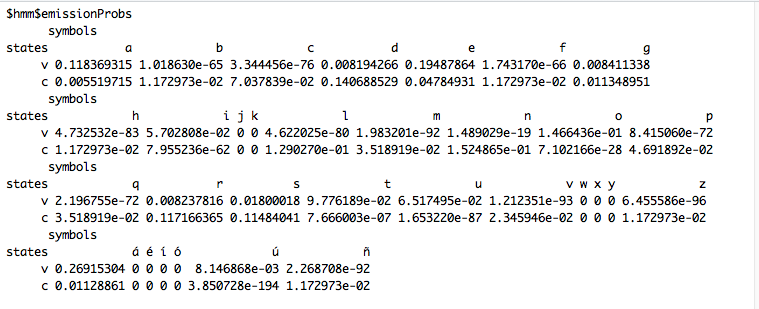
\includegraphics{salida_vocales.png}
\caption{resultados}
\end{figure}

\subsection{Resultados Griego}\label{resultados-griego}

Inicial sin conocimiento:

\begin{longtable}[c]{@{}ccc@{}}
\toprule\addlinespace
& V & C
\\\addlinespace
\midrule\endhead
& 0.53765 & 0.4234
\\\addlinespace
\bottomrule
\end{longtable}

Inicial después de Baum-Welch

\begin{longtable}[c]{@{}ccc@{}}
\toprule\addlinespace
& V & C
\\\addlinespace
\midrule\endhead
& 0.6117 & 0.3882
\\\addlinespace
\bottomrule
\end{longtable}

Transiciones sin conocimiento

\begin{longtable}[c]{@{}ccc@{}}
\toprule\addlinespace
& V & C
\\\addlinespace
\midrule\endhead
V & 0.3558 & 0.6441
\\\addlinespace
C & 0.5161 & 0.4838
\\\addlinespace
\bottomrule
\end{longtable}

Transiciones después de Baum-Welch

\begin{longtable}[c]{@{}ccc@{}}
\toprule\addlinespace
& V & C
\\\addlinespace
\midrule\endhead
V & 0.0093 & 0.9906
\\\addlinespace
C & 0.6178 & 0.3821
\\\addlinespace
\bottomrule
\end{longtable}

En griego las vocales corresponden a los símbolos:

\begin{longtable}[c]{@{}cc@{}}
\toprule\addlinespace
Griego & ~Vocal
\\\addlinespace
\midrule\endhead
A,$\alpha$ & a
\\\addlinespace
E,$\epsilon$ & e
\\\addlinespace
I,$\iota$ & i
\\\addlinespace
O,$\omicron$ & o
\\\addlinespace
Y,$\upsilon$ & u
\\\addlinespace
\bottomrule
\end{longtable}

A continuación se identifican que las probabilides en el estado \emph{v}
de los símbolos
$\alpha$,$\epsilon$,$\iota$,$\omicron$,$\upsilon$,$\epsilon$ acentuado,
son mayores que las probabilidades de estos símbolos al estado \emph{c}.
De igual forma, las probabilidades en el estado \emph{c} para los
símbolos que \textbf{no} son
$\alpha$,$\epsilon$,$\iota$,$\omicron$,$\upsilon$,$\epsilon$ acentuado
son mayores que las probabilidades de estos símbolos al estado \emph{v}.

\begin{figure}[htbp]
\centering
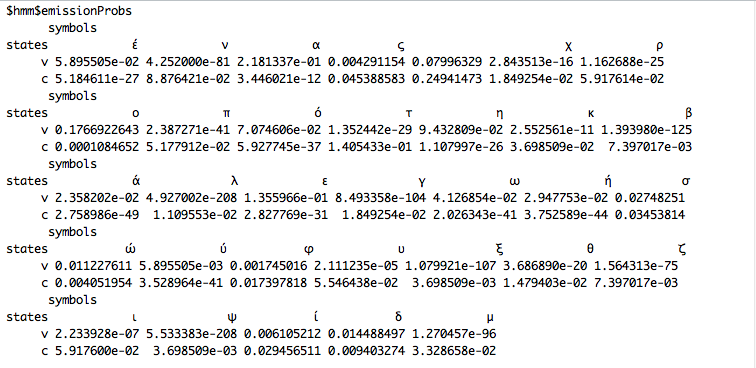
\includegraphics{salida_vocales_griego.png}
\caption{resultados}
\end{figure}

\pagebreak

\subsection{Código}\label{codigo}

\subsubsection{Español}\label{espanol}

\begin{Shaded}
\begin{Highlighting}[]
\KeywordTok{library}\NormalTok{(HMM)}

\NormalTok{periodico <-}\StringTok{ }\KeywordTok{scan}\NormalTok{(}\DataTypeTok{file=}\StringTok{'./datos/Es_Newspapers.txt'}\NormalTok{, }\DataTypeTok{sep=}\StringTok{"}\CharTok{\textbackslash{}n}\StringTok{"}\NormalTok{, }\DataTypeTok{what =} \KeywordTok{character}\NormalTok{())}

\CommentTok{#limpieza de datos}
\NormalTok{for(i in }\DecValTok{1}\NormalTok{:}\KeywordTok{length}\NormalTok{(periodico)) \{}
  \NormalTok{periodico[i] <-}\StringTok{ }\KeywordTok{gsub}\NormalTok{(}\StringTok{"[[:punct:]]"}\NormalTok{,}\StringTok{""}\NormalTok{,}\KeywordTok{unlist}\NormalTok{(periodico[i]))}
  \NormalTok{periodico[i] <-}\StringTok{ }\KeywordTok{gsub}\NormalTok{(}\StringTok{"[[:digit:]]"}\NormalTok{,}\StringTok{""}\NormalTok{,}\KeywordTok{unlist}\NormalTok{(periodico[i]))}
  \NormalTok{periodico[i] <-}\StringTok{ }\KeywordTok{tolower}\NormalTok{(periodico[i])}
  \NormalTok{periodico[i] <-}\StringTok{ }\KeywordTok{gsub}\NormalTok{(}\StringTok{"[[:space:]]"}\NormalTok{,}\StringTok{" "}\NormalTok{,}\KeywordTok{unlist}\NormalTok{(periodico[i]))}
\NormalTok{\}}


\CommentTok{#separando a letras}
\NormalTok{for (i in }\DecValTok{1}\NormalTok{) \{}
  \NormalTok{texto <-}\StringTok{ }\NormalTok{periodico[i]}
  \NormalTok{if(i ==}\StringTok{ }\DecValTok{1}\NormalTok{)\{}
    \NormalTok{obsv <-}\StringTok{ }\KeywordTok{as.data.frame}\NormalTok{(}\KeywordTok{unlist}\NormalTok{(}\KeywordTok{strsplit}\NormalTok{(texto, }\DataTypeTok{split=}\StringTok{""}\NormalTok{)), }\DataTypeTok{stringsAsFactors=}\OtherTok{FALSE}\NormalTok{)}
  \NormalTok{\} else \{}
    \NormalTok{obsv <-}\StringTok{ }\KeywordTok{rbind}\NormalTok{(obsv, }\KeywordTok{as.data.frame}\NormalTok{(}\KeywordTok{unlist}\NormalTok{(}\KeywordTok{strsplit}\NormalTok{(texto, }\DataTypeTok{split=}\StringTok{""}\NormalTok{)), }\DataTypeTok{stringsAsFactors=}\OtherTok{FALSE}\NormalTok{))}
  \NormalTok{\}}
\NormalTok{\}}
\KeywordTok{names}\NormalTok{(obsv) <-}\StringTok{ "letter"}


\NormalTok{states =}\StringTok{ }\KeywordTok{c}\NormalTok{(}\StringTok{"v"}\NormalTok{,}\StringTok{"c"}\NormalTok{)}
\NormalTok{symbols =}\StringTok{ }\KeywordTok{c}\NormalTok{(}\StringTok{"a"}\NormalTok{,}\StringTok{"b"}\NormalTok{,}\StringTok{"c"}\NormalTok{,}\StringTok{"d"}\NormalTok{,}\StringTok{"e"}\NormalTok{,}\StringTok{"f"}\NormalTok{,}\StringTok{"g"}\NormalTok{,}\StringTok{"h"}\NormalTok{,}\StringTok{"i"}\NormalTok{,}\StringTok{"j"}\NormalTok{,}\StringTok{"k"}\NormalTok{,}\StringTok{"l"}\NormalTok{,}\StringTok{"m"}\NormalTok{,}\StringTok{"n"}\NormalTok{,}\StringTok{"o"}\NormalTok{,}\StringTok{"p"}\NormalTok{,}\StringTok{"q"}\NormalTok{,}\StringTok{"r"}\NormalTok{,}
            \StringTok{"s"}\NormalTok{,}\StringTok{"t"}\NormalTok{,}\StringTok{"u"}\NormalTok{,}\StringTok{"v"}\NormalTok{,}\StringTok{"w"}\NormalTok{,}\StringTok{"x"}\NormalTok{,}\StringTok{"y"}\NormalTok{,}\StringTok{"z"}\NormalTok{,}\StringTok{" "}\NormalTok{,}\StringTok{"á"}\NormalTok{,}\StringTok{"é"}\NormalTok{,}\StringTok{"í"}\NormalTok{,}\StringTok{"ó"}\NormalTok{,}\StringTok{"ú"}\NormalTok{,}\StringTok{"ñ"}\NormalTok{)}
\CommentTok{#probabilidades iniciales de lso estados}
\NormalTok{random_num <-}\StringTok{ }\KeywordTok{runif}\NormalTok{(}\DecValTok{1}\NormalTok{,}\FloatTok{0.5}\NormalTok{,}\FloatTok{0.7}\NormalTok{)}
\NormalTok{startProbs =}\StringTok{ }\KeywordTok{matrix}\NormalTok{(}\KeywordTok{c}\NormalTok{(random_num, }\DecValTok{1}\NormalTok{-random_num), }\DecValTok{2}\NormalTok{)}

\NormalTok{random_num <-}\StringTok{ }\KeywordTok{runif}\NormalTok{(}\DecValTok{1}\NormalTok{, }\FloatTok{0.5}\NormalTok{,}\FloatTok{0.7}\NormalTok{)}
\NormalTok{random_num_2 <-}\StringTok{ }\KeywordTok{runif}\NormalTok{(}\DecValTok{1}\NormalTok{, }\FloatTok{0.5}\NormalTok{,}\FloatTok{0.7}\NormalTok{)}
\NormalTok{transProbs <-}\StringTok{ }\KeywordTok{matrix}\NormalTok{(}\KeywordTok{c}\NormalTok{(}\DecValTok{1}\NormalTok{-random_num, random_num_2, }
                       \NormalTok{random_num, }\DecValTok{1}\NormalTok{-random_num_2), }\DecValTok{2}\NormalTok{)}
  
\NormalTok{random_nums <-}\StringTok{ }\KeywordTok{data.frame}\NormalTok{(}\KeywordTok{runif}\NormalTok{(}\DecValTok{33}\NormalTok{,}\FloatTok{0.030}\NormalTok{,}\FloatTok{0.034}\NormalTok{), }\KeywordTok{runif}\NormalTok{(}\DecValTok{33}\NormalTok{,}\FloatTok{0.030}\NormalTok{,}\FloatTok{0.034}\NormalTok{))}
\NormalTok{random_nums <-}\StringTok{ }\KeywordTok{data.frame}\NormalTok{(}\KeywordTok{rep}\NormalTok{(}\DecValTok{1}\NormalTok{/}\DecValTok{33}\NormalTok{,}\DecValTok{33}\NormalTok{), }\KeywordTok{rep}\NormalTok{(}\DecValTok{1}\NormalTok{/}\DecValTok{33}\NormalTok{,}\DecValTok{33}\NormalTok{))}
\NormalTok{emissionProbs=}\KeywordTok{as.matrix}\NormalTok{(random_nums)}
\NormalTok{inithmm <-}\StringTok{ }\KeywordTok{initHMM}\NormalTok{(states, symbols, }\DataTypeTok{startProbs=}\NormalTok{startProbs, }\DataTypeTok{transProbs=}\NormalTok{transProbs, }
                   \DataTypeTok{emissionProbs=}\NormalTok{emissionProbs)}
\NormalTok{bw <-}\StringTok{ }\KeywordTok{baumWelch}\NormalTok{(inithmm, obsv$letter)}
\NormalTok{bw}
\end{Highlighting}
\end{Shaded}

\subsubsection{Griego}\label{griego}

\begin{Shaded}
\begin{Highlighting}[]
\KeywordTok{library}\NormalTok{(HMM)}

\KeywordTok{setwd}\NormalTok{(}\StringTok{"/Users/Lili/Documents/itam/estadistica_multivariada_y_datos_categoricos/examenes/final"}\NormalTok{)}


\NormalTok{periodico <-}\StringTok{ }\KeywordTok{scan}\NormalTok{(}\DataTypeTok{file=}\StringTok{'griego_test.txt'}\NormalTok{, }\DataTypeTok{sep=}\StringTok{"}\CharTok{\textbackslash{}n}\StringTok{"}\NormalTok{, }\DataTypeTok{what =} \KeywordTok{character}\NormalTok{())}



\NormalTok{for(i in }\DecValTok{1}\NormalTok{:}\KeywordTok{length}\NormalTok{(periodico)) \{}
  \NormalTok{periodico[i] <-}\StringTok{ }\KeywordTok{gsub}\NormalTok{(}\StringTok{"[[:punct:]]"}\NormalTok{,}\StringTok{""}\NormalTok{,}\KeywordTok{unlist}\NormalTok{(periodico[i]))}
  \NormalTok{periodico[i] <-}\StringTok{ }\KeywordTok{gsub}\NormalTok{(}\StringTok{"[[:digit:]]"}\NormalTok{,}\StringTok{""}\NormalTok{,}\KeywordTok{unlist}\NormalTok{(periodico[i]))}
  \NormalTok{periodico[i] <-}\StringTok{ }\KeywordTok{tolower}\NormalTok{(periodico[i])}
  \NormalTok{periodico[i] <-}\StringTok{ }\KeywordTok{gsub}\NormalTok{(}\StringTok{"[[:space:]]"}\NormalTok{,}\StringTok{" "}\NormalTok{,}\KeywordTok{unlist}\NormalTok{(periodico[i]))}
\NormalTok{\}}



\NormalTok{for (i in }\DecValTok{1}\NormalTok{) \{}
  \NormalTok{texto <-}\StringTok{ }\NormalTok{periodico[i]}
  \NormalTok{if(i ==}\StringTok{ }\DecValTok{1}\NormalTok{)\{}
    \NormalTok{obsv <-}\StringTok{ }\KeywordTok{as.data.frame}\NormalTok{(}\KeywordTok{unlist}\NormalTok{(}\KeywordTok{strsplit}\NormalTok{(texto, }\DataTypeTok{split=}\StringTok{""}\NormalTok{)), }\DataTypeTok{stringsAsFactors=}\OtherTok{FALSE}\NormalTok{)}
  \NormalTok{\} else \{}
    \NormalTok{obsv <-}\StringTok{ }\KeywordTok{rbind}\NormalTok{(obsv, }\KeywordTok{as.data.frame}\NormalTok{(}\KeywordTok{unlist}\NormalTok{(}\KeywordTok{strsplit}\NormalTok{(texto, }\DataTypeTok{split=}\StringTok{""}\NormalTok{)), }\DataTypeTok{stringsAsFactors=}\OtherTok{FALSE}\NormalTok{))}
  \NormalTok{\}}
\NormalTok{\}}
\KeywordTok{names}\NormalTok{(obsv) <-}\StringTok{ "letter"}

\CommentTok{#obsv <- obsv[-which(obsv$letter=="¾"),]}
\CommentTok{#obsv <- obsv[-which(obsv == "å")]}

\NormalTok{states =}\StringTok{ }\KeywordTok{c}\NormalTok{(}\StringTok{"v"}\NormalTok{,}\StringTok{"c"}\NormalTok{)}
\NormalTok{symbols =}\StringTok{ }\KeywordTok{c}\NormalTok{(}\StringTok{"έ"}\NormalTok{,}\StringTok{"ν"}\NormalTok{,}\StringTok{"α"}\NormalTok{,}\StringTok{"ς"}\NormalTok{,}\StringTok{" "}\NormalTok{,}\StringTok{"χ"}\NormalTok{,}\StringTok{"ρ"}\NormalTok{,}\StringTok{"ο"}\NormalTok{,}\StringTok{"π"}\NormalTok{,}\StringTok{"ό"}\NormalTok{,}\StringTok{"τ"}\NormalTok{,}\StringTok{"η"}\NormalTok{,}\StringTok{"κ"}\NormalTok{,}\StringTok{"β"}\NormalTok{,}\StringTok{"ά"}\NormalTok{,}\StringTok{"λ"}\NormalTok{,}\StringTok{"ε"}\NormalTok{,}\StringTok{"γ"}\NormalTok{,}\StringTok{"ω"}\NormalTok{,}\StringTok{"ή"}\NormalTok{,}\StringTok{"σ"}\NormalTok{,}\StringTok{"ώ"}\NormalTok{,}\StringTok{"ύ"}\NormalTok{,}\StringTok{"φ"}\NormalTok{,}\StringTok{"υ"}
            \NormalTok{,}\StringTok{"ξ"}\NormalTok{,}\StringTok{"θ"}\NormalTok{,}\StringTok{"ζ"}\NormalTok{,}\StringTok{"ι"}\NormalTok{,}\StringTok{"ψ"}\NormalTok{,}\StringTok{"ί"}\NormalTok{,}\StringTok{"δ"}\NormalTok{,}\StringTok{"μ"}\NormalTok{)}
\CommentTok{#probabilidades iniciales de lso estados}
\NormalTok{random_num <-}\StringTok{ }\KeywordTok{runif}\NormalTok{(}\DecValTok{1}\NormalTok{,}\FloatTok{0.5}\NormalTok{,}\FloatTok{0.7}\NormalTok{)}
\NormalTok{startProbs =}\StringTok{ }\KeywordTok{matrix}\NormalTok{(}\KeywordTok{c}\NormalTok{(random_num, }\DecValTok{1}\NormalTok{-random_num), }\DecValTok{2}\NormalTok{)}

\NormalTok{random_num <-}\StringTok{ }\KeywordTok{runif}\NormalTok{(}\DecValTok{1}\NormalTok{, }\FloatTok{0.5}\NormalTok{,}\FloatTok{0.7}\NormalTok{)}
\NormalTok{random_num_2 <-}\StringTok{ }\KeywordTok{runif}\NormalTok{(}\DecValTok{1}\NormalTok{, }\FloatTok{0.5}\NormalTok{,}\FloatTok{0.7}\NormalTok{)}
\NormalTok{transProbs <-}\StringTok{ }\KeywordTok{matrix}\NormalTok{(}\KeywordTok{c}\NormalTok{(}\DecValTok{1}\NormalTok{-random_num,random_num_2,  }
                       \NormalTok{random_num,}\DecValTok{1}\NormalTok{-random_num_2), }\DecValTok{2}\NormalTok{)}
  
\CommentTok{#random_nums <- data.frame(runif(31,0.030,0.034), runif(33,0.030,0.034))}
\NormalTok{random_nums <-}\StringTok{ }\KeywordTok{data.frame}\NormalTok{(}\KeywordTok{rep}\NormalTok{(}\DecValTok{1}\NormalTok{/}\KeywordTok{length}\NormalTok{(symbols),}\KeywordTok{length}\NormalTok{(symbols)), }\KeywordTok{rep}\NormalTok{(}\DecValTok{1}\NormalTok{/}\KeywordTok{length}\NormalTok{(symbols),}\KeywordTok{length}\NormalTok{(symbols)))}
\NormalTok{emissionProbs=}\KeywordTok{as.matrix}\NormalTok{(random_nums)}
\NormalTok{inithmm <-}\StringTok{ }\KeywordTok{initHMM}\NormalTok{(states, symbols, }\DataTypeTok{startProbs=}\NormalTok{startProbs, }\DataTypeTok{transProbs=}\NormalTok{transProbs, }
                   \DataTypeTok{emissionProbs=}\NormalTok{emissionProbs)}
\NormalTok{bw <-}\StringTok{ }\KeywordTok{baumWelch}\NormalTok{(inithmm, obsv$letter)}
\NormalTok{bw}
\end{Highlighting}
\end{Shaded}

\pagebreak

\subsection{Bibliografía}\label{bibliografia}

\end{document}
